\chapter{Stabiliteit en maximale belading}
\label{chap:stabiliteit}

Dit hoofdstuk stelt de stabiliteit van \emph{'t~Jansje} in lege conditie vast en
bepaalt het \emph{maximaal toe te voegen gewicht} voordat de stabiliteits- of
diepgangseis wordt overschreden. Daarmee legt het de gewichtsgrens vast waarbinnen
de daadwerkelijke ontwerpconfiguraties moeten passen; die configuraties worden
zelf doorgerekend in het hoofdstuk Eindontwerp. Alle berekeningen zijn uitgevoerd
voor zoetwater ($\rho = 1000\ \mathrm{kg/m^3}$), omdat \emph{'t~Jansje}
voornamelijk vaart op de Nieuwe Maas.

% ============================================================
\section{Scheepsgegevens en invoer}
\label{sec:stab_geometrie}

\begin{table}[H]
\centering
\caption{Invoerparameters stabiliteitsberekening}
\label{tab:stab_input}
\begin{tabular}{llll}
\toprule
Parameter & Symbool & Waarde & Eenheid \\
\midrule
\multicolumn{4}{l}{\textit{Scheepsgegevens}} \\
\midrule
Lengte waterlijn            & $L$      & 22{,}22 & m     \\
Maximale breedte            & $B$      &  4{,}36 & m     \\
Gemiddelde diepgang (leeg)  & $T$      &  1{,}50 & m     \\
Rompdiepte (kiel t/m dek)   & $D$      &  2{,}05 & m     \\
Verdringingsvolume (leeg)   & $\nabla$ & 73{,}0  & m$^3$ \\
Scheepsgewicht (leeg)       & $W$      & 73{,}0  & t     \\
Waterplancoëfficiënt        & $C_{WP}$ &  0{,}795& --    \\
\bottomrule
\end{tabular}
\end{table}

% --- Sectie "Batterijpakking" (200-cellen vulling) verwijderd:
%     de daadwerkelijke batterijconfiguraties worden doorgerekend in het
%     hoofdstuk Eindontwerp. Dit hoofdstuk bepaalt enkel lege conditie + gewichtsgrens. ---

% ============================================================
\section{Stabiliteitsberekening}
\label{sec:stab_berekening}

De initiële dwarsscheepse stabiliteit wordt bepaald door de metacentrische
hoogte \cite[p.~44]{Barras2006}:

\begin{equation}
    GM = KB + BM - KG \geq 0{,}15\ \mathrm{m}
    \label{eq:GM}
\end{equation}

\subsection{Lege conditie}

\paragraph{Hoogte drijfpunt $KB$}
Voor scheepsvormige vaartuigen geldt $KB \approx 0{,}535 \times T$
\cite[p.~104]{Barras2006}:

\begin{equation}
    KB = 0{,}535 \times 1{,}50 = 0{,}803\ \mathrm{m}
\end{equation}

\paragraph{Metacentrische straal $BM$}
Het tweede moment van het waterplan wordt benaderd via
\cite[Hfst.~1]{Schneekluth1998}:

\begin{equation}
    I_T = \frac{L\,B^3}{12}\!\left(0{,}096 + 0{,}89\,C_{WP}^2\right)
        = \frac{22{,}22 \times 4{,}36^3}{12}
          \!\left(0{,}096 + 0{,}89 \times 0{,}795^2\right)
        = 101{,}1\ \mathrm{m^4}
\end{equation}

\begin{equation}
    BM = \frac{I_T}{\nabla} = \frac{101{,}1}{73{,}0} = 1{,}384\ \mathrm{m}
    \qquad \cite[p.~107]{Barras2006}
\end{equation}

\paragraph{Zwaartepunt $KG$}
Voor \emph{'t~Jansje} is geen hellingsproef  uitgevoerd, waardoor $KG$ niet
direct bekend is. Omdat $KG$ afhangt van hoe het gewicht van het schip
verdeeld is over de constructie, is er ook geen algemene formule om het te
berekenen uit de hoofdafmetingen alleen.

Om toch een uitspraak te kunnen doen over de stabiliteit, is in
Tabel~\ref{tab:KG_gevoeligheid} berekend hoe $GM$ verandert voor
verschillende waarden van $KG$. Hieruit blijkt dat $GM$ pas onder het
IMO-minimum van 0{,}15~m zakt bij $KG > 2{,}04$~m. Dat is vrijwel gelijk
aan de rompdiepte ($D = 2{,}05$~m), wat fysisch onmogelijk is: het
zwaartepunt van het schip kan nooit hoger liggen dan het dek. Het schip
voldoet dus aan de stabiliteitseis voor elke realistische massaverdeling.
Voor de verdere berekening wordt $KG_\mathrm{leeg} = 1{,}30$~m aangehouden.

\begin{table}[H]
\centering
\caption{Gevoeligheid van $GM_\mathrm{leeg}$ voor de aanname van $KG$
         ($KM = KB + BM = 2{,}187$~m)}
\label{tab:KG_gevoeligheid}
\small
\begin{tabular}{ccc}
\toprule
$KG_\mathrm{leeg}$ [m] & $GM_\mathrm{leeg}$ [m] & Beoordeling \\
\midrule
1{,}00 & 1{,}187 & Ruim voldoende \\
1{,}10 & 1{,}087 & Ruim voldoende \\
1{,}20 & 0{,}987 & Ruim voldoende \\
\rowcolor{yellow!20}
1{,}30 & 0{,}887 & Ruim voldoende \\
1{,}50 & 0{,}687 & Voldoende \\
1{,}70 & 0{,}487 & Voldoende \\
1{,}90 & 0{,}287 & Voldoende \\
2{,}04 & 0{,}147 & Grenswaarde ($\approx$ IMO-minimum) \\
\bottomrule
\end{tabular}
\vspace{4pt}

\noindent\footnotesize
\textit{Gele rij: gehanteerde rekenwaarde. IMO-minimum: $GM \geq 0{,}15$~m.}
\end{table}

De metacentrische hoogte in lege conditie bedraagt daarmee:

\begin{equation}
    GM_\mathrm{leeg} = 0{,}803 + 1{,}384 - 1{,}30 = \boxed{0{,}887\ \mathrm{m}}
    \label{eq:GM_leeg}
\end{equation}

\subsection{Maximaal toe te voegen gewicht}
\label{subsec:max_belading}

Het maximaal toe te voegen gewicht wordt begrensd door twee onafhankelijke
eisen: de \emph{diepgangs-/vrijboordeis} en de \emph{IMO-eis voor de
metacentrische hoogte} ($GM \geq 0{,}15$~m). Hieronder wordt voor beide de
bijbehorende grensmassa bepaald; de kleinste van de twee is bindend. De
berekening gebruikt een wandverticale benadering met constant waterplanoppervlak
\begin{equation}
    A_{WP} = C_{WP} \cdot L \cdot B
           = 0{,}795 \times 22{,}22 \times 4{,}36
           = 77{,}0\ \mathrm{m^2},
\end{equation}
en $I_T = 101{,}1\ \mathrm{m^4}$ constant, zoetwater
($\rho = 1000\ \mathrm{kg/m^3}$), een vrijboordmarge van $0{,}20$~m en een
zwaartepunt van de toegevoegde lading op $z_\mathrm{lad} = 1{,}20$~m boven kiel.

\paragraph{Eis 1 -- diepgang/vrijboord.}
De maximale diepgang is $T_\mathrm{max} = D - 0{,}20 = 1{,}85$~m,
zodat het schip nog $\Delta T = 1{,}85 - 1{,}50 = 0{,}35$~m mag inzakken.
Het gewicht van het daarmee extra verplaatste water geeft de grensmassa:

\begin{equation}
    M_{\mathrm{max},T} = \Delta T \times \rho \cdot A_{WP}
                   = 0{,}35 \times 1000 \times 77{,}0 \times 10^{-3}
                   = \boxed{27{,}0\ \mathrm{t}}
    \label{eq:Mmax}
\end{equation}

\paragraph{Eis 2 -- IMO-stabiliteit ($GM \geq 0{,}15$~m).}
Met de toegevoegde massa $M$ veranderen diepgang, drijfpunt, metacenterstraal
en zwaartepunt mee:

\begin{equation}
    GM(M) = \underbrace{0{,}535\!\left(1{,}50 + \tfrac{M}{77{,}0}\right)}_{KB(M)}
          + \underbrace{\frac{101{,}1}{73{,}0 + M}}_{BM(M)}
          - \underbrace{\frac{73{,}0 \times 1{,}30 + M \times 1{,}20}{73{,}0 + M}}_{KG(M)}
    \label{eq:GM_vanM}
\end{equation}

Bij de diepgangsgrens ($M = 27{,}0$~t, $T = 1{,}85$~m) levert dit:

\begin{equation}
    GM(27{,}0) = 0{,}990 + 1{,}011 - 1{,}273 = 0{,}728\ \mathrm{m}.
\end{equation}

Over het hele toelaatbare bereik blijft $GM$ vrijwel constant rond
$0{,}73$--$0{,}89$~m (zie Figuur~\ref{fig:GM_vs_M}) en zakt het nooit in de
buurt van het IMO-minimum van $0{,}15$~m. De GM-eis wordt pas overschreden bij
een $KG$ boven $2{,}04$~m (Tabel~\ref{tab:KG_gevoeligheid}), wat fysisch
onmogelijk is. De stabiliteit levert dus geen praktische bovengrens op.

\paragraph{Bindende eis.}
De diepgangs-/vrijboordeis (Eis~1) is bindend met
$M_\mathrm{max} = 27{,}0$~t; de IMO-GM-eis (Eis~2) wordt ruim gehaald. Bij de
grensmassa is $GM = 0{,}728$~m, nog altijd ruim boven het minimum. De
daadwerkelijke batterijconfiguraties (ordegrootte $1{,}8$--$2{,}2$~t, zie het
hoofdstuk Eindontwerp) vallen hiermee ruimschoots, ruim een factor~$10$, onder
dit maximum.

\paragraph{Langsscheepse stabiliteit}
Het tweede moment om de dwarsscheepse as bedraagt
$I_L = C_{WP} \cdot BL^3/12 = 3169\ \mathrm{m^4}$, wat een langsscheepse
metacentrische hoogte geeft van:

\begin{equation}
    GM_L = KB + \frac{I_L}{\nabla} - KG
         = 0{,}803 + 43{,}4 - 1{,}30
         = 42{,}9\ \mathrm{m}
\end{equation}

Dit is een factor $\sim 48$ groter dan de dwarsscheepse $GM$ en is voor een
centraal geplaatste lading niet de beperkende factor.

% ============================================================
\section{Figuren}
\label{sec:stab_figuren}

\begin{figure}[H]
\centering
\begin{tikzpicture}[
    >=Stealth, scale=2.2,
    punkt/.style={circle, fill=#1, draw=#1!70!black, inner sep=2.2pt},
    lbl/.style={font=\small\bfseries, text=#1}
]
\def\Bhalf{2.0}
\def\D{2.05}
\def\T{1.50}
\def\KB{0.803}
\def\KG{1.300}
\def\KM{2.187}

\fill[blue!12] (-\Bhalf-0.3,0) rectangle (\Bhalf+0.3,\T);
\fill[blue!28, opacity=0.7] (-\Bhalf,0) rectangle (\Bhalf,\T);
\draw[blue!60!black, dashed, semithick]
    (-\Bhalf-0.4,\T) -- (\Bhalf+0.4,\T)
    node[right, font=\tiny, text=blue!70!black] {WL};
\draw[black, line width=1.6pt]
    (-\Bhalf,\D) -- (-\Bhalf,0) -- (\Bhalf,0) -- (\Bhalf,\D);
\draw[gray!40, thin, dashed] (0,-0.18) -- (0,2.55);

\node[punkt=black!80]       at (0,0)    {};
\node[punkt=blue!70!black]  at (0,\KB)  {};
\node[punkt=red!75!black]   at (0,\KG)  {};
\node[punkt=green!55!black] at (0,\KM)  {};

\node[lbl=black,           anchor=east] at (-0.10,0)    {$K$};
\node[lbl=blue!70!black,   anchor=east] at (-0.10,\KB)  {$B$};
\node[lbl=red!75!black,    anchor=east] at (-0.10,\KG)  {$G$};
\node[lbl=green!55!black,  anchor=east] at (-0.10,\KM)  {$M$};

\node[font=\tiny, text=blue!70!black,  anchor=west] at (0.08,\KB) {0{,}803~m};
\node[font=\tiny, text=red!75!black,   anchor=west] at (0.08,\KG) {1{,}300~m};
\node[font=\tiny, text=green!55!black, anchor=west] at (0.08,\KM) {2{,}187~m};

\draw[<->, thick, blue!60!black]
    (-0.65,0) -- (-0.65,\KB)
    node[midway, left, font=\scriptsize, text=blue!60!black] {$KB=0{,}803$~m};
\draw[<->, thick, orange!80!black]
    (-0.65,\KB) -- (-0.65,\KM)
    node[midway, left, font=\scriptsize, text=orange!80!black] {$BM=1{,}384$~m};
\draw[<->, thick, purple!80!black]
    (0.62,\KB) -- (0.62,\KG)
    node[midway, right, font=\scriptsize, text=purple!80!black] {$BG=0{,}497$~m};
\draw[<->, thick, green!55!black]
    (0.62,\KG) -- (0.62,\KM)
    node[midway, right, font=\scriptsize, text=green!55!black] {$GM=0{,}887$~m};

\draw[<->] (-\Bhalf,-0.14) -- (\Bhalf,-0.14)
    node[midway, below, font=\scriptsize] {$B = 4{,}36$~m};
\draw[<->] (\Bhalf+0.32,0) -- (\Bhalf+0.32,\T)
    node[midway, right, font=\scriptsize] {$T=1{,}50$~m};
\draw[<->] (\Bhalf+0.55,0) -- (\Bhalf+0.55,\D)
    node[midway, right, font=\scriptsize] {$D=2{,}05$~m};
\end{tikzpicture}
\caption{Dwarsdoorsnede van \emph{'t~Jansje} in lege conditie
         ($KG = 1{,}30$~m als rekenwaarde). $GM = 0{,}887$~m.}
\label{fig:stab_dwarsdoorsnede_leeg}
\end{figure}

\begin{figure}[H]
\centering
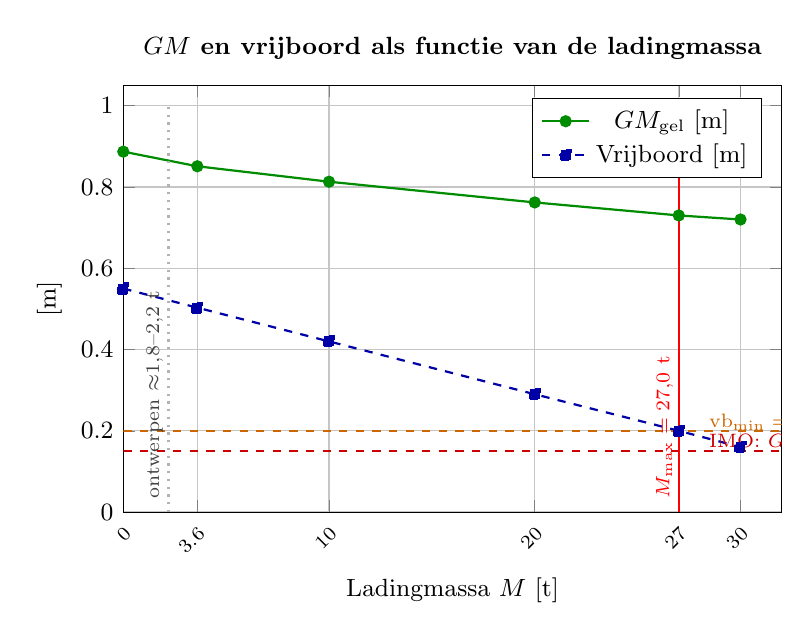
\begin{tikzpicture}
\begin{axis}[
    width=0.82\textwidth, height=7.0cm,
    xlabel={Ladingmassa $M$ [t]},
    ylabel={[m]},
    title={$GM$ en vrijboord als functie van de ladingmassa},
    xmin=0, xmax=32, ymin=0, ymax=1.05,
    xtick={0,3.6,10,20,27,30},
    xticklabel style={font=\scriptsize, rotate=45, anchor=north east},
    grid=both,
    grid style={line width=0.3pt, draw=gray!25},
    major grid style={line width=0.5pt, draw=gray!45},
    legend pos=north east, legend style={font=\small},
    tick label style={font=\small}, label style={font=\small},
    title style={font=\small\bfseries},
]
\addplot[green!55!black, thick, mark=*, mark size=1.8pt] coordinates {
    (0,0.887)(3.6,0.851)(10,0.813)(20,0.762)(27,0.730)(30,0.720)
};
\addlegendentry{$GM_\mathrm{gel}$ [m]}

\addplot[blue!65!black, thick, dashed, mark=square*, mark size=1.8pt] coordinates {
    (0,0.550)(3.6,0.503)(10,0.420)(20,0.290)(27,0.200)(30,0.160)
};
\addlegendentry{Vrijboord [m]}

\addplot[red!80!black, dashed, thick, forget plot]
    coordinates {(0,0.15)(32,0.15)};
\node[red!80!black, font=\scriptsize, anchor=west]
    at (axis cs:28,0.17) {IMO: $GM \geq 0{,}15$~m};

\addplot[orange!80!black, dashed, thick, forget plot]
    coordinates {(0,0.20)(32,0.20)};
\node[orange!80!black, font=\scriptsize, anchor=west]
    at (axis cs:28,0.22) {vb$_\mathrm{min}=0{,}20$~m};

\addplot[red, thick, forget plot] coordinates {(27,0)(27,1.0)};
\node[red, font=\scriptsize, rotate=90, anchor=south west]
    at (axis cs:27.2,0.01) {$M_\mathrm{max}=27{,}0$~t};

\addplot[gray!60, thick, dotted, forget plot] coordinates {(2.2,0)(2.2,1.0)};
\node[gray!50!black, font=\scriptsize, rotate=90, anchor=south west]
    at (axis cs:2.4,0.01) {ontwerpen $\approx$1{,}8--2{,}2~t};
\end{axis}
\end{tikzpicture}
\caption{$GM$ en vrijboord als functie van de ladingmassa ($KG_\mathrm{leeg}
         = 1{,}30$~m). De rode verticale lijn markeert de bindende
         vrijboordlimiet van 27{,}0~t. De daadwerkelijke ontwerpladingen
         ($\approx$1{,}8--2{,}2~t, hoofdstuk Eindontwerp) vallen ver
         binnen beide criteria.}
\label{fig:GM_vs_M}
\end{figure}

% ============================================================
\section{Overzicht resultaten}
\label{sec:stab_overzicht}

\begin{table}[H]
\centering
\caption{Stabiliteitsoverzicht \emph{'t~Jansje} -- lege conditie en bij de
         maximale (bindende) ladingmassa}
\label{tab:stab_overzicht}
\begin{tabular}{lrrl}
\toprule
Grootheid & Leeg & Bij $M_\mathrm{max}$ ($27$~t) & Eenheid \\
\midrule
Diepgang $T$             & 1{,}500 & 1{,}850 & m     \\
Vrijboord                & 0{,}550 & 0{,}200 & m     \\
$\nabla$                 & 73{,}0  & 100{,}0 & m$^3$ \\
\midrule
$KB$                     & 0{,}803 & 0{,}990 & m \\
$BM$                     & 1{,}384 & 1{,}011 & m \\
$KG$                     & 1{,}300 & 1{,}273 & m \\
\midrule
\rowcolor{green!15}
$GM$                     & \textbf{0{,}887} & \textbf{0{,}728} & m \\
IMO-minimum $GM$         & \multicolumn{2}{c}{0{,}150} & m \\
CCR-minimum $GM$ \cite{CCR2015} & \multicolumn{2}{c}{0{,}300} & m \\
\bottomrule
\end{tabular}
\end{table}

% --- Sectie "Beperkingen" verplaatst naar het hoofdstuk Discussie (zie Discussie.tex) ---
% (label sec:stab_beperkingen verhuist mee)

% ============================================================
\section*{Conclusie}
\label{sec:stab_conclusie}

In lege conditie bedraagt de metacentrische hoogte $GM = 0{,}887$~m, ruim
boven het IMO-minimum van $0{,}15$~m. Het maximaal toe te voegen gewicht wordt
begrensd door de diepgangs-/vrijboordeis op $M_\mathrm{max} = 27{,}0$~t; bij die
grensmassa is $GM$ nog $0{,}728$~m, zodat de dwarsscheepse stabiliteit nooit de
bindende factor is. De daadwerkelijke ontwerpladingen ($\approx 1{,}8$--$2{,}2$~t,
zie hoofdstuk Eindontwerp) blijven hier ruimschoots onder.